\begin{homeworkProblem}[8][Graph for 8(c)]
Since the stability criteria don't include $a$, to make plotting
easier, the constant $a$ is set to be $1$. All the initial values are set to be 
5, just for convenience. The steady states were marked by a magenta horizontal
line in each picture.
\begin{figure}[htbp]
\begin{subfigure}[t]{0.45\linewidth}
    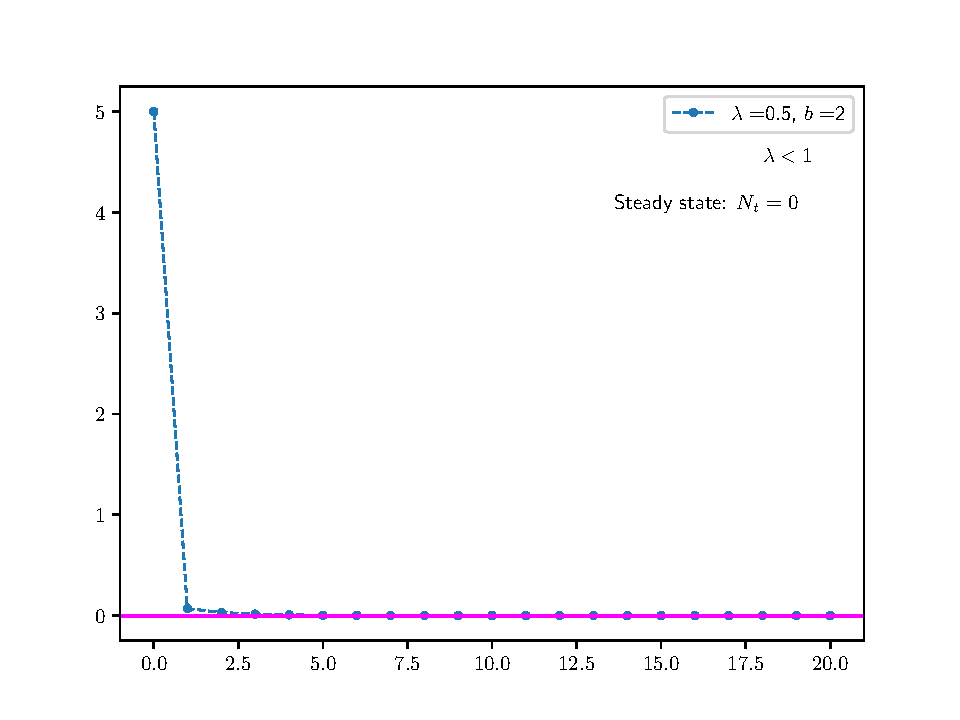
\includegraphics[scale = 0.5]{fig/fig8(c)(1).pdf}
    \caption{$\lambda < 1$, satisfying the stability
    condition for steady state $\bar N = 0$}
\end{subfigure}
\hfill
\begin{subfigure}[t]{0.45\linewidth}
    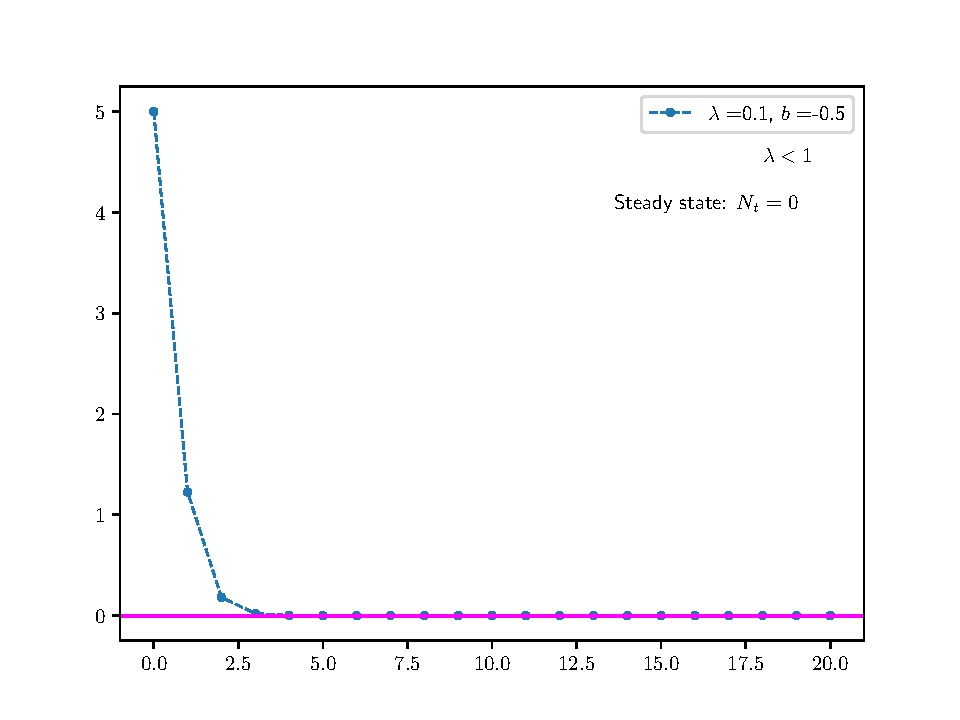
\includegraphics[scale = 0.5]{fig/fig8(c)(2).pdf}
    \caption{$\lambda < 1$, satisfying the stability
    condition for steady state $\bar N = 0$}
\end{subfigure}
\\
\begin{subfigure}[t]{0.45\linewidth}
    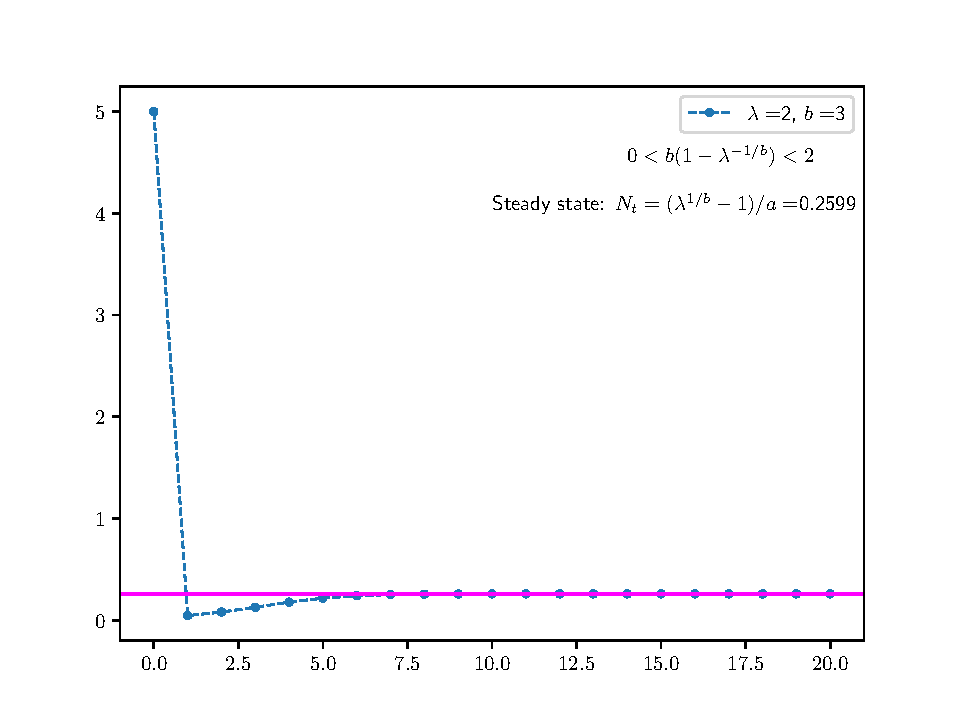
\includegraphics[scale = 0.5]{fig/fig8(c)(3).pdf}
    \caption{$0 < b(1-\lambda^{-1/b})<2$, satisfying the stability
    condition for steady state $\bar N = (\lambda^{1/b} - 1)/a$}
\end{subfigure}
\hfill
\begin{subfigure}[t]{0.45\linewidth}
    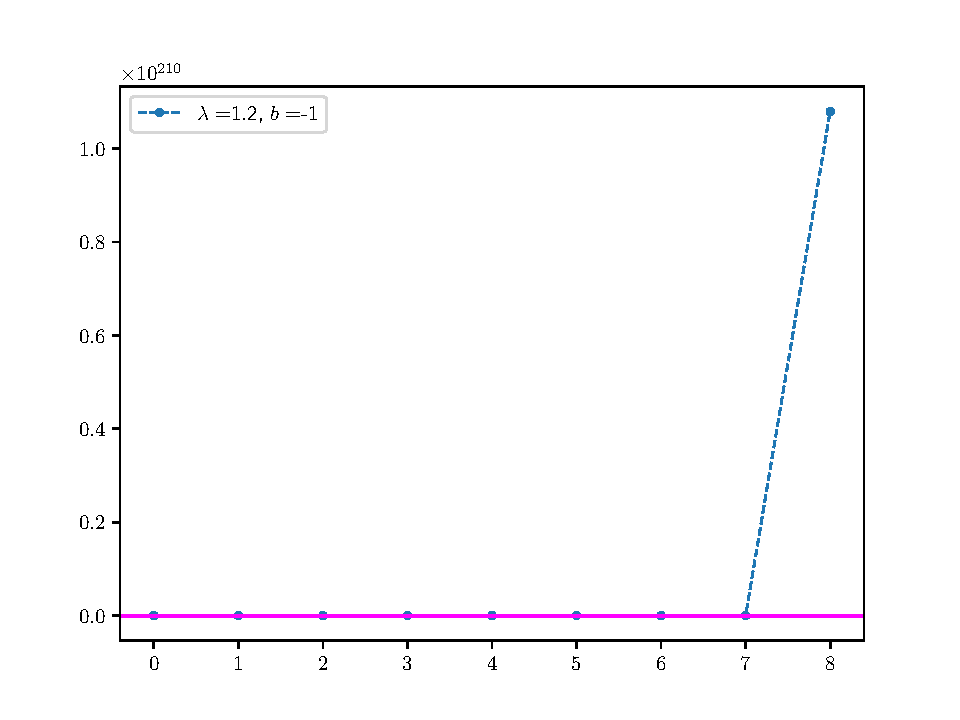
\includegraphics[scale = 0.5]{fig/fig8(c)(4).pdf}
    \caption{No stable steady state, resulting in steep growth (This can be 
    observed from the y axis tick unit: $1.0*10^{210}$. And $N_t$ after 
    $t = 8$ even causes a RuntimeWarning saying the values are not finite!)}
\end{subfigure}
\caption{Graphs for 4 different sets of $\lambda$ and $b$}
\end{figure}
\end{homeworkProblem}